\chapter{Project Architecture}
\section{Component Diagram}
\pagebreak
 \begin{figure}[H]
\centering
 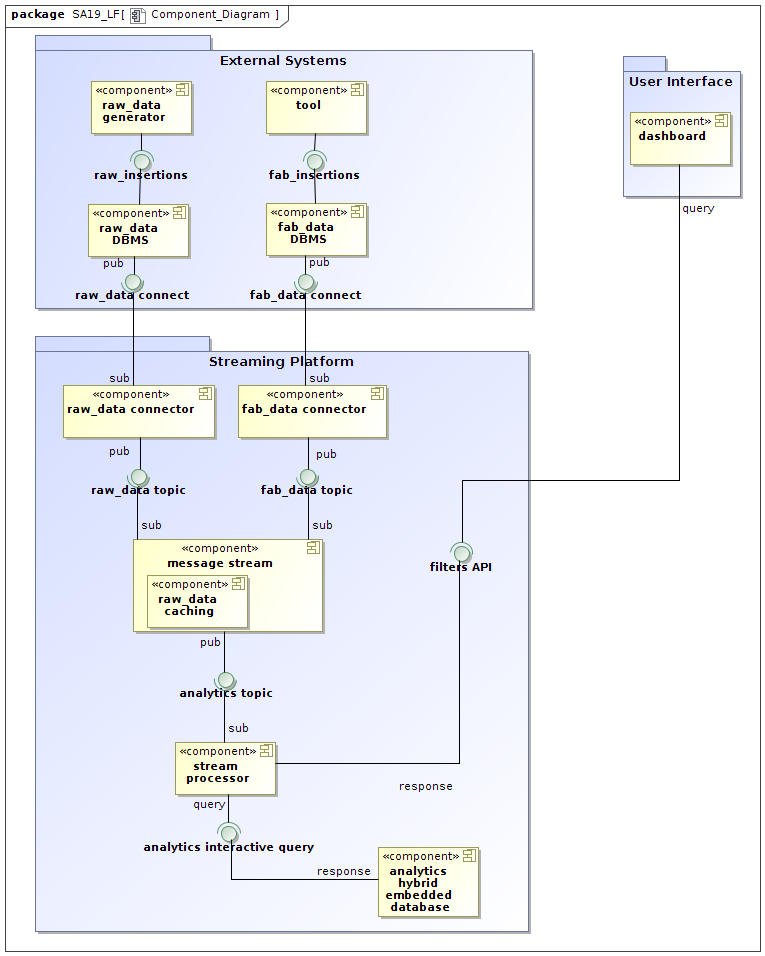
\includegraphics[width=\textwidth, height=\textheight]{img/Component_Diagram.png}
\caption{Component diagram.}
\end{figure}

\subsection{Components Description}
\begin{itemize}
    \item External Systems Package: This package contains the external databases and systems which our system depends upon.
    This package represents everything that is provided by the customer.
    \begin{itemize}
        \item \textbf{raw\_data DBMS}: This component refers to the external database raw\textunderscore data.
        \item \textbf{fab\_data DBMS}: This component refers to the external database fab\textunderscore data.
        \item \textbf{raw\_data generator}: This component refers to an external system that inserts data into the external database raw\_data.
        \item \textbf{tool}: This component refers to the external tool that generates events and inserts them into the fab\textunderscore data database.
    \end{itemize}
    \item Streaming Platform Package:
    \begin{itemize}
        \item \textbf{fab\textunderscore data connector}: This component is responsible for streaming the event messages (received by the external fab\textunderscore data database via a specific tool interface) into a Kafka topic called fab\_data topic.
        \item \textbf{raw\textunderscore data connector}: This component is responsible for streaming the translation messages (received by the external raw\textunderscore data database via a specific tool interface) into a Kafka topic called raw\_data topic.
        \item \textbf{message stream}: This component is subscribed to two topics: fab\_data topic \& raw\_data topic. It is responsible for the translation of the fab\_data events. In order to do this, this component uses internal caching.
        \item \textbf{raw\_data caching}: This component is used to cache the information taken from the raw\_data database by using raw\_data topic. It caches  the latest pair (OID, nameTranslation) received for each id (which could be eqipOID, recipeOID, stepOID). Therefore it allows for a raw\_data:fab\_data relationship in the system of 1:n.
        \item \textbf{stream processor}: This component does the following:
        \begin{itemize}
            \item consumes translated information from the specific topics and stores them into the analytics DBMS, both the Kafka one and the MongoDB one.
            \item applies both default and user-specified filters to the analytics information.
            \item sends requests to the analytics DBMS according to some of the filters (for getting past information).
            \item provides the analytics information (past and current) to the dashboard.
        \end{itemize}
        \item \textbf{analytics hybrid embedded database}: This component is responsible for the storage of the tools' information.
    \end{itemize}
    \item User Interface Package:
    \begin{itemize}
        \item \textbf{dashboard}: This component is responsible for the visualization of the stored information. Also it allows the final user to apply specific filters on the requested data. 
    \end{itemize}

\end{itemize}

\subsection{Interfaces Description}
\begin{itemize}
    \item External Database Package:
    \begin{itemize}
        \item \textbf{raw insertions}: This interface represent the communication between the raw\_data generator and the raw\_data DBMS. 
        \item \textbf{fab insertions}: This interface represent the tool(s) and fab\_data DBMS. 
        \item \textbf{raw\_data connect}: This interface is responsible for the communication between the external database raw\textunderscore data and our system. This communication is discrete, and happens on demand by our system.
        \item \textbf{fab\_data connect}: This interface is responsible for the communication between the external database fab\textunderscore data and our system. This communication has to be in real-time, as soon as a new entry is inserted into the database this interface has to provide it to our system.
    \end{itemize}
    \item Streaming Platform Package:
    \begin{itemize}
        \item \textbf{fab\_data topic}: This interface refers to all the topics that are used by the component fab\textunderscore data connector to stream the external fab\textunderscore data database.
        \item \textbf{raw\_data topic}: This interface refers to all the topics that are used by the component raw\textunderscore data connector to stream the external raw\textunderscore data database.
        \item \textbf{analytics topic}: This interface refers to all the topics in which the translated information are written so that the component \textit{message stream} can store them.
         \item \textbf{analytics interactive queries}: This interface performs CRUD operations with the analytics DBMS.
    \end{itemize}
    \item Analytics Package:
    \begin{itemize}
        \item \textbf{filters API}: This interface is responsible for the communication between the user's dashboard and our system.
    \end{itemize}
\end{itemize}

\section{Sequence Diagram}

\subsection{Dashboard}

This diagram represents the actions' flow of a query made by an end user on the dashboard. This component will send a message to the stream processor component, which is responsible of the analytics message flow. If the time concerning the query is the present, it means that the end user is interested in some part of the flow which is passing through the stream processor at the current moment, and the processor will consume the interested data; otherwise, it will send a MakeQuery() message to the hybrid embedded analytics database, located in our system. In this database all the analytics data are stored, and it's where the system will search to answer queries about past information.
In both cases, the dashboard will receive a return.


\begin{figure}[H]
\centering
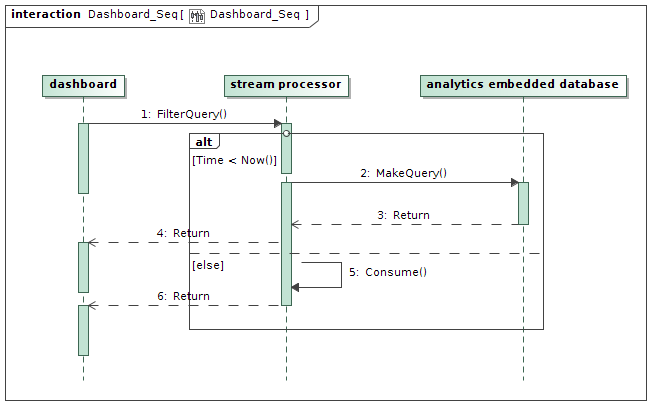
\includegraphics[width=\textwidth]{img/Dashboard_Seq.png}
\caption{Sequence diagram from the \textbf{dashboard} point of view.}
\end{figure}

\subsection{Raw\_data}
This diagram represents the events that occur when the raw\_data generator inserts new data into the database. Of course, this means that it will send an Insert message to the raw\_data DBMS, which in turn will publish this value on its Kafka topic, namely the raw\_data connect, at which the raw\_data connector is subscribed and in turn will send a consume operation. After that the raw\_data connector will publish the processed message in the raw\_data topic.

\begin{figure}[H]
\centering
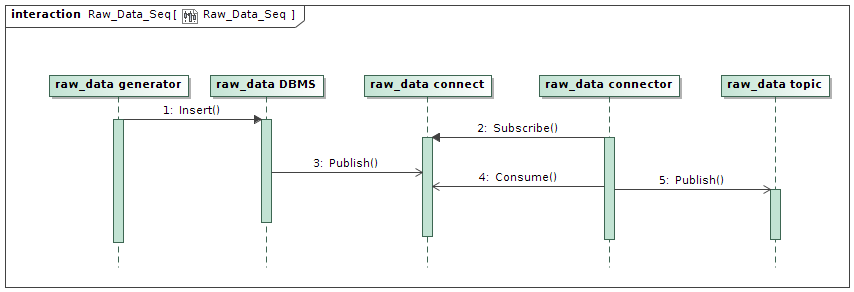
\includegraphics[width=\textwidth]{img/Raw_Data_Seq.png}
\caption{Sequence diagram from the \textbf{raw\_data} point of view.}
\end{figure}

\subsection{Fab\_data}

\begin{figure}[H]
\centering
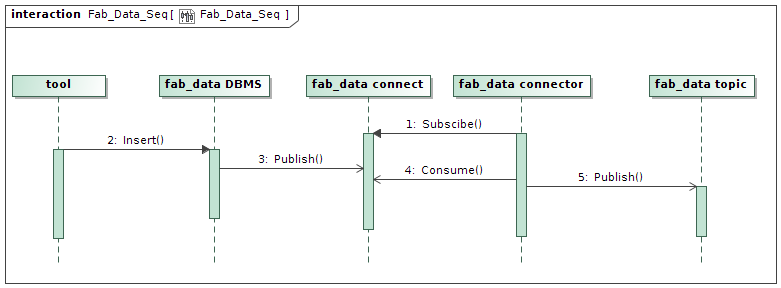
\includegraphics[width=\textwidth]{img/Fab_Data_Seq.png}
\caption{Sequence diagram from the \textbf{fab\_data} point of view.}
\end{figure}

This diagram represents the events that occur when a tool inserts an event into the external database. When this happens the fab\_data connector (which was subscribed to that topic) receives the new event and, after some computation, publishes it in the new fab\_data topics.

\subsection{Streaming}
\begin{figure}[H]
\centering
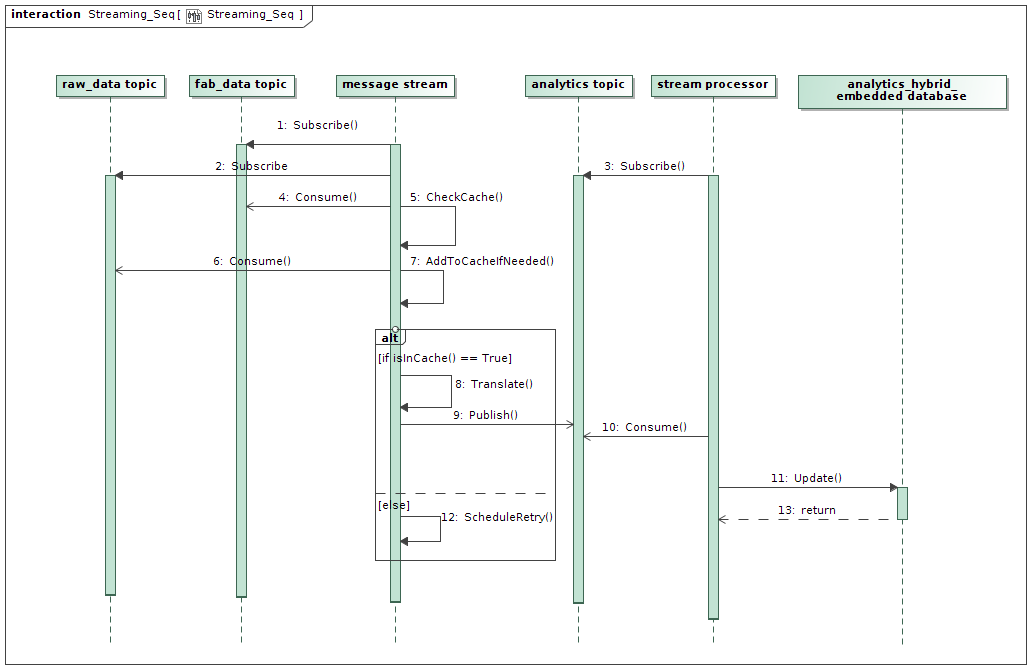
\includegraphics[width=\textwidth]{img/Streaming_Seq.png}
\caption{Sequence diagram of the \textbf{Streaming platform} flow of events.}
\end{figure}

This diagram represent the actions taken by the streaming platfrom package. the \textit{Message Stream} subscribes to both fab\_data and raw\_data topics then when there is a publication of a new message on the fab\_data topic, the message is consumed by the message stream. Then the message stream compares the OID in the message to its cache, if a recipe with that OID is not present, it stores this failed translation into a specific kafka topic and it delays the translation so that it can retry later (every 30 sec). Else if the information are present, this component performs the translation and republishes the result into a specific output topics in the analytics\_topics interface. This message is consumed my the stream processor that stores it both in the kafka DB and, by using kafka connect, also in the external database.